\section{Cooling Towers and Evaporative Fluid Coolers }\label{cooling-towers-and-evaporative-fluid-coolers}

\subsection{One, Two, and Variable Speed Cooling Towers and Evaporative Fluid Coolers}\label{one-two-and-variable-speed-cooling-towers-and-evaporative-fluid-coolers}

\subsubsection{Overview}\label{overview-012}

The input objects CoolingTower:SingleSpeed, CoolingTower:TwoSpeed, and CoolingTower:VariableSpeed:Merkel provide models for single-speed, two-speed, and variable-speed cooling towers that are based on Merkel's theory (Merkel 1925), which is also the basis for the tower model included in ASHRAE's HVAC1 Toolkit for primary HVAC system energy calculations (ASHRAE 1999, Bourdouxhe et al. 1994). Cooling tower performance is modeled using effectiveness-NTU relationships for counterflow heat exchangers. The model can be used to simulate the performance of both single speed, two speed, and variable speed mechanical-draft cooling towers. The model will also account for tower performance in the ``free convection'' regime, when the tower fan is off but the water pump remains on. For part-load operation, the model assumes a simple linear interpolation between two steady-state regimes without accounting for any cycling losses.

For single speed cooling towers, the capacity control can be fan cycling or fluid bypass. In fluid bypass mode, portion of the water goes through the tower media and gets cooled while the remaining water flow gets bypassed, two water flows then mix together trying to meet the tower exiting water setpoint temperature. In both the free convection cooling when fan is off and normal cooling when fan is on for the entire time step, if the tower exiting water temperature is lower than the setpoint, the tower operates in fluid bypass mode. The model determines the fluid bypass fraction by iterations until the mixed water meets the tower exiting water temperature setpoint. In the fluid bypass mode, except the free convection, the tower fan runs at full speed for the entire time step. The maximum amount of tower water that can be bypassed is bounded by the freezing point of the tower water -- the tower exiting water temperature cannot be lower than the freezing setpoint.

Evaporative fluid coolers are modeled very similar to cooling towers. The main difference between the two is in the ``Performance input method'' input field. Cooling tower has two choices for this field namely ``UFactorTimesAreaAndDesignWaterFlowRate'' and ``Nominal capacity''. The nominal capacity is specified for the standard conditions i.e.~entering water at 35\(^{\circ}\)C (95\(^{\circ}\)F), leaving water at 29.44\(^{\circ}\)C (85\(^{\circ}\)F), entering air at 25.56\(^{\circ}\)C (78\(^{\circ}\)F) wet-bulb temperature and 35\(^{\circ}\)C (95\(^{\circ}\)F) dry-bulb temperature. On the other hand evaporative fluid cooler has three choices for ``Performance input method'' which are ``UFactorTimesAreaAndDesignWaterFlowRate'', ``StandardDesignCapacity'' and ``UserSpecifiedDesignCapacity''. First method is same for both tower and fluid cooler. Standard design capacity is specified for the same conditions which are used to specify nominal capacity for tower as described above. If the capacity of fluid cooler for conditions other than the standard ones is known then UserSpecifiedDesignCapacity method should be used. In this case, the conditions for which the fluid cooler capacity is known i.e.~entering water temperature, entering air temperature and entering air wet bulb temperature must be specified in the input. To calculate evaporation loss for fluid cooler, spray water flow rate which is different than the process fluid flow rate must be specified for all the performance input methods. This is not required for cooling tower because cooled fluid i.e.~water is in direct contact with the air so the water loss is calculated by using cooled fluid flow rate only. Unlike cooling tower, evaporative fluid cooler model does not account for free convection.

Cooling tower model is described below which holds equally good for evaporative fluid cooler. The differences are mentioned whenever required.

\subsubsection{Model Description}\label{model-description-008}

Based on Merkel's theory, the steady-state total heat transfer between the air and water entering the tower can be defined by the following equation:

\begin{equation}
d{\dot Q_{total}} = \frac{{UdA}}{{c_p}}\left( {{h_s} - {h_a}} \right)
\label{eq:MerkelTheorySteadyStateQtotal}
\end{equation}

where:

\emph{h\(_{s}\)} is the enthalpy of saturated air at the wetted-surface temperature (J/kg)

\emph{h\(_{a}\)} is the enthalpy of air in the free stream (J/kg)

\emph{c\(_{p}\)} is the specific heat of moist air (J/kg-\(^{\circ}\)C)

\emph{U} is the cooling tower overall heat transfer coefficient (W/m\(^{2}\)-\(^{\circ}\)C)

\emph{A} is the heat transfer surface area (m\(^{2}\)).

Equation~\ref{eq:MerkelTheorySteadyStateQtotal} is based on several assumptions:

\begin{itemize}
\item air and water vapor behave as ideal gases

\item the effect of water evaporation is neglected

\item fan heat is neglected

\item the interfacial air film is assumed to be saturated

\item the Lewis number is equal to 1

\end{itemize}

In this model, it is also assumed that the moist air enthalpy is solely a function of the wet-bulb temperature and that the moist air can be treated as an equivalent ideal gas with its mean specific heat defined by the following equation:

\begin{equation}
\bar c_{pe} = \frac{{\Delta h}}{{\Delta {T_{wb}}}}
\label{eq:cpebardeltahdeltaTwb}
\end{equation}

where:

\(\Delta h\) is the enthalpy difference between the air entering and leaving the tower (J/kg)

\(\Delta T_{wb}\) is the wet-bulb temperature difference between the air entering and leaving the tower (\(^{\circ}\)C).

Since the liquid side conductance is much greater than the gas side conductance, the wetted-surface temperature is assumed to be equal to the water temperature. Based on this assumption and Equations~\ref{eq:MerkelTheorySteadyStateQtotal} and~\ref{eq:cpebardeltahdeltaTwb}, the expression for total heat transfer becomes:

\begin{equation}
d{\dot Q_{total}} = U_e dA\left( {{T_w} - {T_{wb}}} \right)
\label{eq:dQtotal509}
\end{equation}

where:

\begin{equation}
U_e = \frac{{U\,\bar c_{pe}}}{{cp}}
\end{equation}

\(T_{wb}\) is the wet-bulb temperature of the air (\(^{\circ}\)C)

\emph{T\(_{w}\)} is the temperature of the water (\(^{\circ}\)C).

An energy balance on the water and air sides of the air/water interface yields the following equations:

\begin{equation}
d{\dot Q_{total}} = {\dot m_w} c_{pw} dT_w
\label{eq:dQtotal510}
\end{equation}

\begin{equation}
d{\dot Q_{total}} = {\dot m_a} \bar c_{pe} dT_{wb}
\label{eq:dQtotal511}
\end{equation}

where:

\({\dot m_w}\) is the mass flow rate of water (kg/s)

\({\dot m_a}\) is the mass flow rate of air (kg/s).

Assuming that the heat capacity rate (\(\dot mc_p\) ) for the cooling tower water is less than that for the air, the effectiveness of the cooling tower can be defined by analogy to the effectiveness of a simple heat exchanger:

\begin{equation}
\varepsilon  = \frac{{{T_{win}} - {T_{wout}}}}{{{T_{win}} - {T_{wbin}}}}
\label{eq:varepsilon512}
\end{equation}

where

\emph{\(\varepsilon\)} is the heat exchanger effectiveness

\emph{T\(_{win}\)} is the inlet water temperature (\(^{\circ}\)C)

\emph{T\(_{wout}\)} is the outlet water temperature (\(^{\circ}\)C)

\emph{T\(_{wbin}\)} is the wet-bulb temperature of the inlet air (\(^{o\circ}\)C).

Combining Equations~\ref{eq:dQtotal509},~\ref{eq:dQtotal510}, and~\ref{eq:dQtotal511} and integrating over the entire heat transfer surface area, and combining the result with Equation~\ref{eq:varepsilon512} provides the following expression for cooling tower effectiveness:

\begin{equation}
\varepsilon = \frac{{1 - \exp \left\{ { - NTU\left[ {1 - \left( {\frac{{{{\dot C}_w}}}{{{{\dot C}_a}}}} \right)} \right]} \right\}}}{{1 - \left( {\frac{{{{\dot C}_w}}}{{{{\dot C}_a}}}} \right)\exp \left\{ { - NTU\left[ {1 - \left( {\frac{{{{\dot C}_w}}}{{{{\dot C}_a}}}} \right)} \right]} \right\}}}
\end{equation}

where:

\begin{equation}
{\dot C_w} = {\dot m_w}c_{pw}
\end{equation}

\begin{equation}
{\dot C_a} = {\dot m_a}\bar c_{pe}
\end{equation}

\begin{equation}
NTU = Number~of~Transfer~Units = \frac{{UA_e}}{{{{\dot C}_w}}}
\end{equation}

This equation is identical to the expression for effectiveness of an indirect contact (i.e., fluids separated by a solid wall) counterflow heat exchanger (Incropera and DeWitt 1981). Therefore, the cooling tower can be modeled, in the steady-state regime, by an equivalent counterflow heat exchanger as shown in the following figure.

\begin{figure}[hbtp] % fig 194
\centering
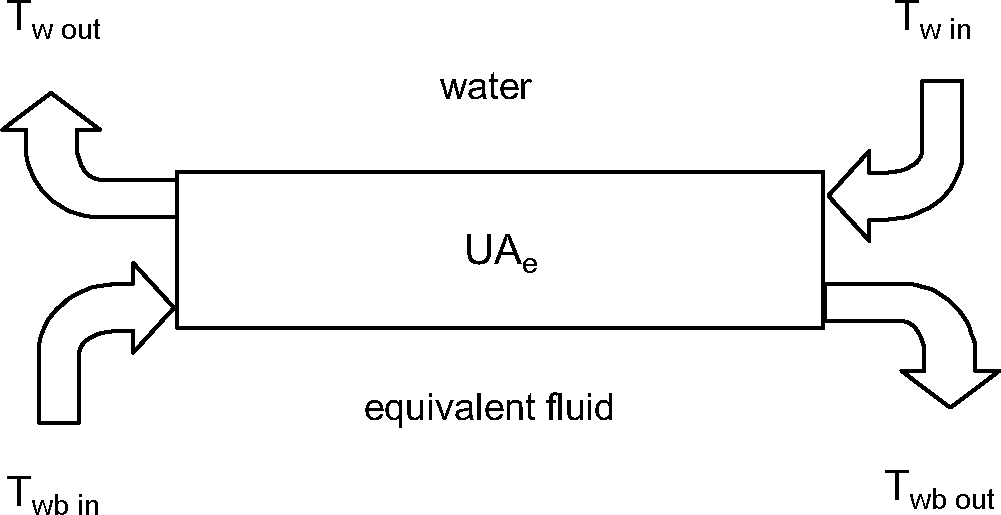
\includegraphics[width=0.9\textwidth, height=0.9\textheight, keepaspectratio=true]{media/image4542.png}
\caption{Cooling Tower Schematic \protect \label{fig:cooling-tower-schematic}}
\end{figure}

The first fluid is water and the second fluid is an equivalent fluid entering the heat exchanger at temperature T\(_{wbin}\) and specific heat \(\bar c_{pe}\). The heat exchanger is characterized by a single parameter, its overall heat transfer coefficient-area product UA\(_{e}\). The actual cooling tower heat transfer coefficient-area product is related to UA\(_{e}\) by the following expression:

\begin{equation}
UA = UA_e\frac{{c_p}}{{\bar c_{pe}}}
\label{eq:UA514}
\end{equation}

This heat transfer coefficient-area product is assumed to be a function of the air mass flow rate only and can be estimated from laboratory test results or manufacturers' catalog data.

The model for the variable speed Merkel tower also includes Scheier's modifications.~ Scheier has extended the Merkel model to also include terms that adjust UA with three factors that model how UA values change when the tower is operating away from its rated conditions.~ The first factor, \({f_{UA,wetbulb}}\) , adjusts UA for the current outdoor wetbulb temperature.~ The user enters a performance curve or lookup table that is a function of one independent variable.~ The independent variable is the difference between the design wetbulb temperature and the current wetbulb temperature, in degrees Celsius.

\begin{equation}
{f_{UA,wetbulb}} = func\left( {\left( {{T_{des,wetbulb}} - {T_{current,wetbulb}}} \right)} \right)
\end{equation}

The second factor, \({f_{UA,airflow}}\), adjusts UA for the current air flow rate.~ The user enters a performance curve or lookup table that is a function of one independent variable.~ The independent variable is the ratio of the current air flow rate to the design air flow rate at full speed.

\begin{equation}
{f_{UA,airflow}} = func\left( {AirFlowRatio} \right)
\end{equation}

The third factor, \({f_{UA,waterflow}}\), adjusts UA for the current water flow rate.~ The user enters a performance curve or lookup table that is a function of one independent variable.~ The independent variable is the ratio of the current water flow rate to the design water flow rate.

\begin{equation}
{f_{UA,waterflow}} = func\left( {WaterFlowRatio} \right)
\end{equation}

Then the UA value at any given time is calculated using:

\begin{equation}
U{A_e} = U{A_{design}} \bullet {f_{UA,wetbulb}} \bullet {f_{UA,airflow}} \bullet {f_{UA,waterflow}}
\end{equation}

\subsubsection{Method for Calculating Steady-State Exiting Water Temperature}\label{method-for-calculating-steady-state-exiting-water-temperature}

The objective of the cooling tower model is to predict the exiting water temperature and the fan power required to meet the exiting water setpoint temperature. Since only the inlet air and inlet water temperatures are known at any simulation time step, an iterative procedure is required to determine the exiting fluid temperatures using the equations defined in the previous section. In the case of the EnergyPlus model, the iterations are performed to determine the exiting wet-bulb temperature of the air. The exiting water temperature is then calculated based on an energy balance that assumes that the energy absorbed by the air is equivalent to the energy removed from the water. The procedure for calculating the steady-state, exiting air wet-bulb temperature is outlined below.

As explained previously, it is assumed that the moist air enthalpy can be defined by the wet-bulb temperature alone. Therefore, the first step in the procedure is to calculate the enthalpy of moist air entering the cooling tower based on the ambient wet-bulb temperature from the weather file. Since an iterative solution is required, a first guess of the outlet air wet-bulb temperature is then made and the enthalpy of this estimated outlet air wet-bulb temperature is calculated. Based on these inlet and outlet air conditions, the mean specific heat of the air is calculated based on Equation~\ref{eq:cpebardeltahdeltaTwb}, repeated here:

\begin{equation}
\bar c_{pe} = \frac{{\Delta h}}{{\Delta T_{wb}}}
\end{equation}

With the overall heat transfer coefficient-area product for the cooling tower entered by the user, the effective heat transfer coefficient-area product is calculated by rearranging Equation~\ref{eq:UA514}:

\begin{equation}
UA_e = UA\frac{{\bar c_{pe}}}{{c_p}}
\end{equation}

With \(\bar c_{pe}\) and \(UA_e\) known, the effectiveness of the heat exchanger is then calculated:

\begin{equation}
\varepsilon \,\, = \,\frac{{1 - \exp \left\{ { - NTU\left[ {1 - \left( {\frac{{{{\dot C}_{\min }}}}{{{{\dot C}_{\max }}}}} \right)} \right]} \right\}}}{{1 - \left( {\frac{{{{\dot C}_{\min }}}}{{{{\dot C}_{\max }}}}} \right)\exp \left\{ { - NTU\left[ {1 - \left( {\frac{{{{\dot C}_{\min }}}}{{{{\dot C}_{\max }}}}} \right)} \right]} \right\}}}
\end{equation}

where:

\begin{equation}
{\dot C_{\min }} = Minimum({\dot C_w},{\dot C_a})
\end{equation}

\begin{equation}
{\dot C_{\max }} = Maximum({\dot C_w},{\dot C_a})
\end{equation}

\begin{equation}
{\dot C_w} = {\dot m_w}c_{pw}
\end{equation}

\begin{equation}
{\dot C_a} = {\dot m_a}\bar c_{pe}
\end{equation}

\begin{equation}
NTU = Number~of~Transfer~Units = \frac{{UAe}}{{{{\dot C}_{\min }}}}
\end{equation}

The heat transfer rate is then calculated as follows:

\begin{equation}
\dot Qtotal = \varepsilon {\dot C_{\min }}\left( {T_{win} - T_{wbin}} \right)
\end{equation}

The outlet air wet-bulb temperature is then recalculated:

\begin{equation}
{T_{wbout}} = {T_{wbin}} + \frac{{{{\dot Q}_{total}}}}{{{{\dot C}_a}}}
\end{equation}

The iterative process of calculating \({T_{wbout}}\) continues until convergence is reached.

Finally, the outlet water temperature is calculated as follows:

\begin{equation}
{T_{wout}} = {T_{win}} + \frac{{{{\dot Q}_{total}}}}{{{{\dot C}_w}}}
\end{equation}

\subsubsection{Calculating the Actual Exiting Water Temperature and Fan Power}\label{calculating-the-actual-exiting-water-temperature-and-fan-power}

The previous section describes the methodology used for calculating the steady-state temperature of the water leaving the cooling tower. This methodology is used to calculate the exiting water temperature in the free convection regime (water pump on, tower fan off) and with the tower fan operating (including low and high fan speed for the two-speed tower). The exiting water temperature calculations use the fluid flow rates (water and air) and the UA-values entered by the user for each regime.

The cooling tower model seeks to maintain the temperature of the water exiting the cooling tower at (or below) a setpoint. The model obtains the target temperature setpoint from the setpoints placed on either the tower outlet node or the loop's overall setpoint node (typically set to the supply side outlet node). The model checks to see if the outlet node has a setpoint placed on it and uses that if it does.~ If the outlet node does not have a temperature setpoint then the model uses the loop-level outlet node specified in the input field called Loop Temperature Setpoint Node Name in the PlantLoop or CondenserLoop object. The model first checks to determine the impact of ``free convection'', if specified by the user, on the tower exiting water temperature. If free convection is not specified by the user, then the exiting water temperature is initially set equal to the entering tower water temperature. If the user specifies ``free convection'' and the steady-state exiting water temperature based on ``free convection'' is at or below the setpoint, then the tower fan is not turned on.

If the exiting water temperature remains above the setpoint after ``free convection'' is modeled, then the tower fan is turned on to reduce the exiting water temperature to the setpoint. The model assumes that part-load operation is represented by a simple linear interpolation between two steady-state regimes (e.g., tower fan on for the entire simulation time step and tower fan off for the entire simulation time step). Cyclic losses are not taken into account.

The fraction of time that the tower fan must operate is calculated based on the following equation:

\begin{equation}
\omega = \frac{{{T_{set}} - {T_{wout,off}}}}{{{T_{wout,on}} - {T_{wout,off}}}}
\label{eq:omegafunctionvariousTs515}
\end{equation}

where:

\({T_{set}}\) is the exiting water setpoint temperature (\(^{\circ}\)C)

\({T_{wout,off}}\) is the exiting water temperature with tower fan off (\(^{\circ}\)C)

\({T_{wout,on}}\) is the exiting water temperature with tower fan on (\(^{\circ}\)C).

The average fan power for the simulation time step is calculated by multiplying \(\omega\) by the steady-state fan power specified by the user.

The calculation method for the two-speed tower is similar to that for the single-speed tower example described above. The model first checks to see if ``free convection'' is specified and if the resulting exiting water temperature is below the setpoint temperature. If not, then the model calculates the steady-state exiting water temperature with the tower fan at low speed. If the exiting water temperature at low fan speed is below the setpoint temperature, then the average fan power is calculated based on the result of Equation~\ref{eq:omegafunctionvariousTs515} and the steady-state, low speed fan power specified by the user. If low-speed fan operation is unable to reduce the exiting water temperature below the setpoint, then the tower fan is increased to its high speed and the steady-state exiting water temperature is calculated. If this temperature is below the setpoint, then a modified version of Equation~\ref{eq:omegafunctionvariousTs515} is used to calculate runtime at high fan speed:

\begin{equation}
\omega \,\, = \frac{{{T_{set}} - {T_{wout,low}}}}{{{T_{wout,high}} - {T_{wout,low}}}}
\end{equation}

where

\({T_{set}}\) is the exiting water setpoint temperature (\(^{\circ}\)C)

\({T_{wout,low}}\) is the exiting water temperature with tower fan at low speed (\(^{\circ}\)C)

\({T_{wout,high}}\) is the exiting water temperature with tower fan at high speed (\(^{\circ}\)C).

The average fan power for the simulation time step is calculated for the two-speed cooling tower as follows:

\begin{equation}
{P_{fan,avg}} = \omega ({P_{fan,high}}) + \left( {1 - \omega } \right)\left( {{P_{fan,low}}} \right)
\end{equation}

The calculation method for the variable-speed Merkel/Scheier model is different from the one- and two-speed models.~ Whereas the other towers are setpoint driven, the variable speed Merkel/Scheier model is driven by the load dispatched from the plant operation scheme, such as PlantEquipmentOperation:CoolingLoad.~ The plant operation scheme provides the cooling tower model with a target load to meet and the tower is controlled to meet that load (as opposed to meeting a leaving setpoint).~ This allows complex configurations with more than one cooling tower to be properly dispatched using all the features available in the various plant operation schemes.~ The model first evaluates the load provided with the fans off using only free convection.~ If the free convection mode meets or exceeds the target load then the tower runs in free convection mode.~ The model then evaluates the load provided by running the fans at full speed.~ If the full fan speed load provided is less than or equal to the target load then the tower runs at full speed.~ The model then evaluates the load provided with the variable speed fan running at the minimum air speed ratio, which is a user input (default is 0.2).~ If the minimum fan speed load provided meets or exceeds the target load, then tower runs at the minimum fan speed.~ If the target load is between the load provided by minimum and maximum fans speeds, then the model solves for an airflow rate ratio that just meets the target load using root solver numerical method.~ The variable speed Merkel/Scheier model does not model bypass and may provided excess cooling at times when running in free convection or at the minimum fan speed.~ Fan power for the variable speed Merkel/Scheier model is then calculated from the airflow rate ratio using a design fan power and a performance curve or lookup table with one independent variable for the airflow ratio.

\begin{equation}
{P_{fan}} = {P_{fan,des}} \bullet func\left( {AirFlowRatio} \right)
\end{equation}

\subsubsection{Tower Basin Heater}\label{tower-basin-heater}

The tower basin heater operates in the same manner as the variable speed cooling tower basin heater. Refer to the variable speed cooling tower basin heater description in the following section.

\subsubsection{Cooling Tower Makeup Water Usage}\label{cooling-tower-makeup-water-usage}

The cooling tower makeup water usage is the same as the variable speed cooling tower makeup water usage. Refer to the variable speed cooling tower makeup water usage description in the following section.

\subsubsection{References}\label{references-015}

Rosaler, Robert C. 1995. Standard Handbook of Plant Engineering, 2\(^{nd}\) Ed. New York, NY: McGraw-Hill, pp.~6-36-37.

\subsection{Variable Speed Cooling Towers Empirical Models}\label{variable-speed-cooling-towers-empirical-models}

\subsubsection{Overview}\label{overview-1-005}

The input object CoolingTower:VariableSpeed provides models for variable speed towers that are based on empirical curve fits of manufacturer's performance data or field measurements. The user specifies tower performance at design conditions, and empirical curves are used to determine the approach temperature and fan power at off-design conditions. The user defines tower performance by entering the inlet air wet-bulb temperature, tower range, and tower approach temperature at the design conditions. The corresponding water flow rate, air flow rate, and fan power must also be specified. The model will account for tower performance in the ``free convection'' regime, when the tower fan is off but the water pump remains on and heat transfer still occurs (albeit at a low level). Basin heater operation and makeup water usage (due to evaporation, drift, and blowdown) are also modeled.

The cooling tower seeks to maintain the temperature of the water exiting the cooling tower at (or below) a setpoint. The setpoint temperature is defined by the setpoints placed on either the tower outlet node or the loop's overall setpoint node (typically set to the supply side outlet node). The model checks to see if the outlet node has a setpoint placed on it and uses that if it does.~ If the outlet node does not have a temperature setpoint then the model uses the loop-level outlet node specified in the input field called Loop Temperature Setpoint Node Name in the PlantLoop or CondenserLoop object. The model simulates the outlet water temperature in four successive steps:

\begin{itemize}
\item The model first determines the tower outlet water temperature with the tower fan operating at maximum speed. If the outlet water temperature is above the setpoint temperature, the fan runs at maximum speed.
\item If the outlet water temperature with maximum fan speed is below the setpoint temperature, then the model next determines the impact of ``free convection'' (water flowing through tower with fan off). If the exiting water temperature based on ``free convection'' is at or below the setpoint, then the tower fan is not turned on.
\item If the outlet water temperature remains above the setpoint after ``free convection'' is modeled, then the tower fan is turned on at the minimum fan speed (minimum air flow rate ratio) to reduce the leaving water temperature. If the outlet water temperature is below the setpoint at minimum fan speed, the tower fan is cycled on and off to maintain the outlet water setpoint temperature.
\item If the outlet water temperature remains above the setpoint after minimum fan speed is modeled, then the tower fan is turned on and the model determines the required air flow rate and corresponding fan speed to meet the desired setpoint temperature.
\end{itemize}

\subsubsection{Model Description}\label{model-description-1-005}

The variable speed tower model utilizes user-defined tower performance at design conditions along with empirical curves to determine tower heat rejection and fan power at off-design conditions. Basin heater operation and makeup water usage are also modeled based on user inputs, tower entering air conditions, and tower operation. The following sections describe how each of these tower performance areas is modeled.

\subsubsection{Tower Heat Rejection}\label{tower-heat-rejection}

Heat rejection by the variable speed cooling tower is modeled based on the CoolTools correlation, YorkCalc correlation, or user-defined coefficients for either the CoolTools or YorkCalc correlations. These purely-empirical correlations model the tower approach temperature using a polynomial curve fit with a large number of terms and either three or four independent variables.

The CoolTools correlation has 35 terms with four independent variables:

\begin{equation}
\begin{array}{rl}
Approach =& Coeff(1) + Coeff(2)•FRair + Coeff(3)•(FRair)^{2} + \\
 & Coeff(4)•(FRair)^{3} + Coeff(5)•FRwater + \\
 & Coeff(6)•FRair•FRwater + Coeff(7)•(FRair)^{2}•FRwater + \\
 & Coeff(8)•(FRwater)^{2} + Coeff(9)•FRair•(FRwater)^{2} + \\
 & Coeff(10)•(FRwater)^{3} + Coeff(11)•Twb + Coeff(12)•FRair•Twb + \\
 & Coeff(13)•(FRair)^{2}•Twb + Coeff(14)•FRwater•Twb + \\
 & Coeff(15)•FRair•FRwater•Twb + Coeff(16)•(FRwater)^{2}•Twb + \\
 & Coeff(17)•(Twb)^{2} + Coeff(18)•FRair•(Twb)^{2} + \\
 & Coeff(19)•FRwater•(Twb)^{2} + Coeff(20)•(Twb)^{3} + Coeff(21)•Tr +  \\
 & Coeff(22)•FRair•Tr + Coeff(23)•(FRair)^{2}•Tr + \\
 & Coeff(24)•FRwater•Tr + Coeff(25)•FRair•FRwater•Tr + \\
 & Coeff(26)•(FRwater)^{2}•Tr + Coeff(27)•Twb•Tr + \\
 & Coeff(28)•FRair•Twb•Tr + Coeff(29)•FRwater•Twb•Tr + \\
 & Coeff(30)•(Twb)^{2}•Tr + Coeff(31)•(Tr)^{2} + Coeff(32)•FRair•(Tr)^{2} + \\
 & Coeff(33)•FRwater•(Tr)^{2} + Coeff(34)•Twb•(Tr)^{2} + Coeff(35)•(Tr)^{3}
\end{array}
\end{equation}

where:

Approach is the approach temperature (\(^{\circ}\)C) which is equal to the outlet water temperature minus the inlet air wet-bulb temperature

FRair is the air flow rate ratio (actual air flow rate divided by design air flow rate)

FRwater is the water flow rate ratio (actual water flow rate divided by design water flow rate)

Tr is the range temperature (\(^{\circ}\)C) which is the inlet water temperature minus the outlet water temperature

Twb is the inlet air wet-bulb temperature (\(^{\circ}\)C)

Coeff(\#) are the correlation coefficients.

If the user selects Tower Model Type = CoolToolsCrossFlow, then the 35 coefficients derived for the CoolTools simulation model (Benton et al. 2002) are used and these coefficients are already defined within EnergyPlus as shown in Table~\ref{table:approach-temperature-correlation-coefficients}. If the user specifies Tower Model Type = CoolToolsUserDefined, then the user must enter a CoolingTowerPerformance:CoolTools object to define the 35 coefficients that will be used by the CoolTools approach temperature correlation.

% table 63
\begin{longtable}[c]{p{2.0in}p{2.0in}p{2.0in}}

\caption{Approach Temperature Correlation Coefficients \label{table:approach-temperature-correlation-coefficients}} \tabularnewline
\toprule 
Coefficient Number & \multicolumn{2}{c}{Coefficient Value} \tabularnewline
\cmidrule(r){2-3}
& CoolTools & YorkCalc \tabularnewline
\midrule
\endfirsthead

\caption[]{Approach Temperature Correlation Coefficients} \tabularnewline
\toprule
Coefficient Number & \multicolumn{2}{c}{Coefficient Value} \tabularnewline
\cmidrule(r){2-3}
& CoolTools & YorkCalc \tabularnewline
\midrule
\endhead

Coeff(1) & 0.52049709836241 & -0.359741205 \tabularnewline
Coeff(2) & -10.617046395344 & -0.055053608 \tabularnewline
Coeff(3) & 10.7292974722538 & 0.0023850432 \tabularnewline
Coeff(4) & -2.74988377158227 & 0.173926877 \tabularnewline
Coeff(5) & 4.73629943913743 & -0.0248473764 \tabularnewline
Coeff(6) & -8.25759700874711 & 0.00048430224 \tabularnewline
Coeff(7) & 1.57640938114136 & -0.005589849456 \tabularnewline
Coeff(8) & 6.51119643791324 & 0.0005770079712 \tabularnewline
Coeff(9) & 1.50433525206692 & -1.342427256E-05 \tabularnewline
Coeff(10) & -3.2888529287801 & 2.84765801111111 \tabularnewline
Coeff(11) & 0.02577861453538 & -0.121765149 \tabularnewline
Coeff(12) & 0.18246428931525 & 0.0014599242 \tabularnewline
Coeff(13) & -0.08189472914009 & 1.680428651 \tabularnewline
Coeff(14) & -0.21501000399629 & -0.0166920786 \tabularnewline
Coeff(15) & 0.01867413096353 & -0.0007190532 \tabularnewline
Coeff(16) & 0.053682417759 & -0.025485194448 \tabularnewline
Coeff(17) & -0.00270968955115 & 4.87491696E-05 \tabularnewline
Coeff(18) & 0.00112277498589 & 2.719234152E-05 \tabularnewline
Coeff(19) & -0.00127758497498 & -0.06537662555556 \tabularnewline
Coeff(20) & 7.60420796601607E-05 & -0.002278167 \tabularnewline
Coeff(21) & 1.43600088336017 & 0.0002500254 \tabularnewline
Coeff(22) & -0.5198695909109 & -0.0910565458 \tabularnewline
Coeff(23) & 0.11733957691051 & 0.00318176316 \tabularnewline
Coeff(24) & 1.50492810819924 & 3.8621772E-05 \tabularnewline
Coeff(25) & -0.13589890592697 & -0.0034285382352 \tabularnewline
Coeff(26) & -0.15257758186651 & 8.56589904E-06 \tabularnewline
Coeff(27) & -0.05338438281146 & -1.516821552E-06 \tabularnewline
Coeff(28) & 0.00493294869566 & N/A \tabularnewline
Coeff(29) & -0.00796260394174 & N/A \tabularnewline
Coeff(30) & 0.00022261982862 & N/A \tabularnewline
Coeff(31) & -0.05439520015681 & N/A \tabularnewline
Coeff(32) & 0.00474266879162 & N/A \tabularnewline
Coeff(33) & -0.01858546718156 & N/A \tabularnewline
Coeff(34) & 0.00115667701294 & N/A \tabularnewline
Coeff(35) & 0.00080737066446 & N/A \tabularnewline
\bottomrule
\end{longtable}

Similarly, the YorkCalc correlation has 27 terms with three independent variables:

\begin{equation}
\begin{array}{rl}
Approach =& Coeff(1) + Coeff(2)•Twb + Coeff(3)•Twb^{2} + Coeff(4)•Tr + \\
 & Coeff(5)•Twb•Tr + Coeff(6)•Twb^{2}•Tr + Coeff(7)•Tr^{2} + \\
 & Coeff(8)•Twb•Tr^{2} + Coeff(9)•Twb^{2}•Tr^{2} + Coeff(10)•LGRatio + \\
 & Coeff(11)•Twb•LGRatio + Coeff(12)•Twb^{2}•LGRatio + \\
 & Coeff(13)•Tr•LGRatio + Coeff(14)•Twb•Tr•LGRatio + \\
 & Coeff(15)•Twb^{2}•Tr•LGRatio + Coeff(16)•Tr^{2}•LGRatio + \\
 & Coeff(17)•Twb•Tr^{2}•LGRatio + Coeff(18)•Twb^{2}•Tr^{2}•LGRatio + \\
 & Coeff(19)•LGRatio^{2} + Coeff(20)•Twb•LGRatio^{2} + \\
 & Coeff(21)• Twb^{2}•LGRatio^{2} + Coeff(22)•Tr•LGRatio^{2} + \\
 & Coeff(23)•Twb•Tr•LGRatio^{2} + Coeff(24)•Twb^{2}•Tr•LGRatio^{2} + \\
 & Coeff(25)•Tr^{2}•LGRatio^{2} + Coeff(26)•Twb•Tr^{2}•LGRatio^{2} + \\
 & Coeff(27)•Twb^{2}•Tr^{2}•LGRatio^{2}
\end{array}
\end{equation}

where:

Approach is the approach temperature (\(^{\circ}\)C) which is the outlet water temperature minus the inlet air wet-bulb temperature

Tr is the range temperature (\(^{\circ}\)C) which is the inlet water temperature minus the outlet water temperature

Twb is the inlet air wet-bulb temperature (\(^{\circ}\)C)

LGratio is the liquid-to-gas ratio which is the ratio of water flow rate ratio (FRwater) to air flow rate ratio (FRair)

Coeff(\#) are the correlation coefficients.

If the user selects Tower Model Type = YorkCalc, then the 27 coefficients derived for the YorkCalc simulation model (York International Corp. 2002) are used and these coefficients are already defined within EnergyPlus as shown in Table~\ref{table:approach-temperature-correlation-coefficients}. If the user specifies Tower Model Type = YorkCalcUserDefined, then the user must enter a CoolingTowerPerformance:YorkCalc object to define the 27 coefficients that will be used by the YorkCalc approach temperature correlation.

The approach temperature correlations for the CoolTools and YorkCalc simulation models are valid for a range of conditions defined in Table~\ref{table:minimum-and-maximum-limits-for-approach}. If the user defines their own model coefficients (CoolingTowerPerformance:CoolTools or CoolingTowerPerformance:YorkCalc), then they must also define in that same object the range of conditions for which the model is valid. For all of these correlation variables, the program issues warnings if the actual values are beyond the minimum/maximum values specified for the correlation being used. For inlet air wet-bulb temperature and water mass flow rate ratio, the values of these variables used in the calculation of approach temperature are limited to be within the valid minimum/maximum range. For approach, range, and liquid-to-gas ratio the warnings are issued if the values are beyond the specified minimum/maximum range but the actual values are still used. The warnings issued do not necessarily indicate a poor estimate of tower performance at the condition(s) which caused the warning, but are provided to identify conditions outside the defined correlation limits. Exceeding the defined limits by a small amount may not introduce significant errors, but large deviations may be problematic. It is for this reason that we recommend using a very broad range of cooling tower performance data (i.e., data covering the entire range expected during the simulation) when generating user-defined coefficients for the variable speed tower model.

% table 64
\begin{longtable}[c]{@{}lll@{}}
\caption{Minimum and Maximum Limits for Approach Temperature Correlation Variables \label{table:minimum-and-maximum-limits-for-approach}} \tabularnewline
\toprule 
Independent Variable Limit & CoolTools & YorkCalc \tabularnewline
\midrule
\endfirsthead

\caption[]{Minimum and Maximum Limits for Approach Temperature Correlation Variables} \tabularnewline
\toprule 
Independent Variable Limit & CoolTools & YorkCalc \tabularnewline
\midrule
\endhead

Minimum Inlet Air Wet-Bulb Temperature & -1.0°C & -34.4°C \tabularnewline
Maximum Inlet Air Wet-Bulb Temperature & 26.7°C & 26.7°C \tabularnewline
Minimum Tower Range Temperature & 1.1°C & 1.1°C \tabularnewline
Maximum Tower Range Temperature & 11.1°C & 22.2°C \tabularnewline
Minimum Tower Approach Temperature & 1.1°C & 1.1°C \tabularnewline
Maximum Tower Approach Temperature & 11.1°C & 40°C \tabularnewline
Minimum Water Flow Rate Ratio & 0.75 & 0.75 \tabularnewline
Maximum Water Flow Rate Ratio & 1.25 & 1.25 \tabularnewline
Maximum Liquid-to-Gas Ratio & N/A & 8.0 \tabularnewline
\bottomrule
\end{longtable}

The approach temperature correlation(s) used to simulate cooling tower heat rejection are based on water and air flow rate ``ratios'' and are not directly dependent on the size of the tower or the actual air and water flow rates through the tower. However, the model correlations are developed based on a reference condition. For Model Types ``CoolToolsCrossFlow'' and ``YorkCalc'', the reference condition is a water flow rate of 0.000043 m\(^{3}\)/s per kW of heat rejected (2.4 gal/min per ton of heat rejected) with 25.6\(^{\circ}\)C (78\(^{\circ}\)F) enter air wet-bulb temperature, 35\(^{\circ}\)C (95\(^{\circ}\)F) hot water inlet temperature, and 29.4\(^{\circ}\)C (85\(^{\circ}\)F) cold water outlet temperature. The reference condition may be different if the user defines tower model coefficients using CoolingTowerPerformance:CoolTools or CoolingTowerPerformance:YorkCalc.

Due to the inherent reference condition used to generate the tower performance curves, the water flow rate at the reference condition must be determined using the design performance information specified by the user and the tower model's approach temperature correlation. This is done by using the model's approach temperature correlation (described earlier in this section) to calculate the water flow rate ratio which yields the user-defined design approach temperature based on an air flow rate ratio of 1.0 (\emph{FR\(_{air}\)} = 1.0), the design inlet air wet-bulb temperature, and the design range temperature. The calculated approach temperature (using the model correlation) must satisfy the following two equations:

\begin{equation}
{T_{water,outlet,design}} = {T_{wb,air,design}} + {T_{approach,design}}\quad \{ F{R_{air}} = 1.0\}
\end{equation}

\begin{equation}
{T_{water,inlet,design}} = {T_{wb,air,design}} + {T_{approach,design}} + {T_{range,design}}\quad \{ F{R_{air}} = 1.0\}
\end{equation}

where:

\({T_{water,outlet,design}}\) is the design outlet water temperature (\(^{\circ}\)C)

\({T_{water,inlet,design}}\) is the design inlet water temperature (\(^{\circ}\)C)

\({T_{wb,air,design}}\) is the design inlet air wet-bulb temperature (\(^{\circ}\)C)

\({T_{approach,design}}\) is the design approach temperature (\(^{\circ}\)C)

\({T_{range,design}}\) is the design range temperature (\(^{\circ}\)C)

\(F{R_{air}}\) is the air flow rate ratio (actual air flow rate divided by design air flow rate).

The water flow rate ratio used in the approach temperature correlation which satisfies these two equations is the ratio of the design water flow rate (specified by the user) to the water flow rate at the reference condition. This ratio is used to calculate the reference water volumetric flow rate, which is then used throughout the simulation to determine the actual water flow rate ratio used in the approach temperature correlation for each simulation time step.

\begin{equation}
{\dot V_{reference}} = \frac{{{{\dot V}_{design}}}}{{F{R_{water,reference}}}}
\end{equation}

where:

\({\dot V_{reference}}\) is the water volumetric flow rate at the reference condition (m\(^{3}\)/s)

\({\dot V_{design}}\) is the design water volumetric flow rate specified by the user (m\(^{3}\)/s)

\(F{R_{water,reference}}\) is the design water flow rate divided by the reference water flow rate.

The cooling tower seeks to maintain the temperature of the water exiting the cooling tower at (or below) a setpoint. The setpoint temperature is defined by the field ``Condenser Loop Temperature Setpoint schedule or reference'' for the CondenserLoop object. The model simulates the outlet water temperature in four successive steps:

\begin{itemize}
\item The model first determines the tower outlet water temperature with the tower fan operating at maximum speed. If the outlet water temperature is above the setpoint temperature, the fan runs at maximum speed.
\item If the outlet water temperature with maximum fan speed is below the setpoint temperature, then the model next determines the impact of ``free convection'' (water flowing through tower with fan off). If the exiting water temperature based on ``free convection'' is at or below the setpoint, then the tower fan is not turned on.
\item If the outlet water temperature remains above the setpoint after ``free convection'' is modeled, then the tower fan is turned on at the minimum fan speed (minimum air flow rate ratio) to reduce the leaving water temperature. If the outlet water temperature is below the setpoint at minimum fan speed, the tower fan is cycled on and off to maintain the outlet water setpoint temperature.
\item If the outlet water temperature remains above the setpoint after minimum fan speed is modeled, then the tower fan is turned on and the model determines the required air flow rate and corresponding fan speed to meet the desired setpoint temperature.
\end{itemize}

For each simulation time step, the model first calculates the outlet water temperature with the tower fan operating at maximum speed (FRair = 1.0). The calculated approach temperature (using the correlations described above), inlet air wet-bulb temperature (weather data), and range temperature are used to determine the tower outlet water temperature as follows:

\begin{equation}
  \begin{array}{rl}
    T_{water,outlet,fanMAX} &= T_{wb,air} + T_{approach} \quad \{FR_{air} = 1.0\} \\
                              &= {T_{water,inlet}} + {T_{range}}
  \end{array}
\end{equation}

where:

\({T_{water,outlet,fanMAX}}\) is the tower outlet water temperature at maximum fan speed (\(^{\circ}\)C)

\({T_{wb,air}}\) is the tower inlet air wet-bulb temperature (\(^{\circ}\)C)

\({T_{approach}}\) is the approach temperature at current operating conditions (\(^{\circ}\)C)

\({T_{range}}\) is the range temperature at current operating conditions (\(^{\circ}\)C).

Note that the approach temperature correlation as described previously is a function of range temperature, so the equations above must be solved iteratively to converge on a solution. If the resulting outlet water temperature is above the desired setpoint temperature, then the fan runs at maximum speed and does not cycle on/off (fan part-load ratio = FanPLR = 1.0 and \emph{FR\(_{air}\)} = 1.0).

If the outlet water temperature with maximum fan speed is below the setpoint temperature, then the model next determines the impact of ``free convection'' (water flowing through tower with fan off). In the free convection regime, the outlet water temperature is calculated using a fraction of the water temperature difference through the tower when the fan is at its maximum speed. This fraction is defined by the user (Fraction of Tower Capacity in Free Convection Regime).

\begin{equation}
{T_{water,outlet,fanOFF}} = {T_{water,inlet}} - \left[ {Fra{c_{freeconv}}\left( {{T_{water,inlet}} - {T_{water,outlet,fanMAX}}} \right)} \right]
\end{equation}

where:

\({T_{water,outlet,fanOFF}}\) is the tower outlet water temperature in free convection regime (\(^{\circ}\)C)

\({T_{water,inlet}}\) is the tower inlet water temperature (\(^{\circ}\)C)

\(Fra{c_{freeconv}}\) is the fraction of tower capacity in free convection regime (user specified).

If the outlet water temperature in the free convection regime is below the setpoint temperature, the tower fan is not turned on and the fan part-load ratio is set equal to 0. In addition, the air flow rate ratio through the tower is assumed to be equal to the fraction of tower capacity in the free convection regime.

\begin{equation}
FanPLR = FanPL{R_{freeconv}} = 0.0
\end{equation}

\begin{equation}
F{R_{air}} = F{R_{air,freeconv}} = Fra{c_{freeconv}}
\end{equation}

where:

\(FanPLR\) is the fan part-load ratio

\(FanPL{R_{freeconv}}\) is the fan part-load ratio in free convection regime

\(F{R_{air,freeconv}}\) is the air flow rate ratio in free convection regime.

If the outlet water temperature in the free convection regime is above the setpoint temperature, then the fan is turned on at the minimum fan speed (minimum air flow rate ratio, FR\(_{air,min}\), entered by the user) and the outlet water temperature is calculated as the inlet air wet-bulb temperature plus the calculated approach temperature:

\begin{equation}
FR_{air} = FR_{air,min}
\end{equation}

\begin{equation}
T_{water,outlet,fanMIN} = T_{wb,air} + T_{approach}
\end{equation}

where:

\({T_{water,outlet,FanMIN}}\)is the outlet water temperature at minimum fan speed (\(^{\circ}\)C)

\(F{R_{air,\min }}\) is the air flow rate ratio at the minimum fan speed.

If the outlet water temperature at minimum fan speed is below the setpoint temperature, the cooling tower fan cycles on and off at the minimum air flow rate ratio in order to meet the setpoint temperature.

\begin{equation}
FanPLR = \left( {\frac{{{T_{water,outlet,fanOFF}} - {T_{setpoint}}}}{{{T_{water,outlet,fanOFF}} - {T_{water,outlet,fanMIN}}}}} \right)
\end{equation}

where \({T_{{\rm{setpoint}}}}\) is the outlet water setpoint temperature (\(^{\circ}\)C).

If the outlet water temperature at minimum fan speed is above the outlet water temperature setpoint, then the cooling tower fan speed (\emph{FR\(_{air}\)}) is increased until the calculated approach temperature produces the required outlet water temperature to meet the setpoint.

\begin{equation}
{T_{approach}} = f\left( {F{R_{air}}} \right)
\end{equation}

\begin{equation}
{T_{water,outlet}} = {T_{{\rm{setpoint}}}} = {T_{wb,air}} + {T_{approach}}
\end{equation}

\begin{equation}
FanPLR = 1.0~~(i.e., fan does not cycle on/off)
\end{equation}

\subsubsection{Fan Power}\label{fan-power}

When the cooling tower fan is operating, fan electric power is calculated based on the air flow rate ratio required to meet the above conditions. If the user has entered a fan power curve object (cubic curve), the output of that curve is multiplied by the design fan power. Otherwise, tower fan power is assumed to be directly proportional to the cube of the air flow rate ratio. In either case, the fan part-load ratio is applied to account for times when the tower fan cycles on/off to meet the setpoint temperature. Fan energy consumption is calculated each simulation time step.

If FanPowerCurveObject is defined, then:

\begin{equation}
  P_{fan} = \left( {CurveOutput} \right)\left( {FanPLR} \right){P_{fan,design}}
\end{equation}

Else:

\begin{equation}
  P_{fan} = \left( {{P_{fan,design}}} \right)\left( {FanPLR} \right){\left( {F{R_{air}}} \right)^{\rm{3}}}
\end{equation}

In addition:

\begin{equation}
{E_{fan}} = \left( {{P_{fan}}} \right)\left( {TimeStepSys} \right)3600
\end{equation}

where:

\(FanPowerCurveObject\) is the name of fan power ratio as a function of air flow rate ratio curve

\({P_{fan}}\) is the tower fan electric power (W)

\({E_{fan}}\) is the tower fan electric consumption (J)

\(CurveOutput\) is the output of FanPowerCurveObject evaluated at the operating air flow rate ratio (\emph{FR\(_{air}\)})

\({P_{fan,design}}\) is the design fan power at design (maximum) air flow through the tower (W)

\emph{TimeStepSys} is the HVAC system simulation time step (hr).

\subsubsection{Tower Basin Heater}\label{tower-basin-heater-1}

Calculations are also made to estimate the electric power input to the tower basin heater. A schedule may be used to disable the basin heater during regular maintenance periods or other time periods (e.g., during summer). If a schedule is not provided, the basin heater is assumed to be available the entire simulation time period. The basin heater operates when it is scheduled on, the outdoor air dry-bulb temperature is below the basin heater setpoint temperature, and the cooling tower is not active (i.e., water is not flowing through the tower). The user is required to enter a basin heater capacity (Watts per degree Kelvin) and a heater setpoint temperature (\(^{\circ}\)C) if they want to model basin heater electric power.

\begin{lstlisting}
P_heater_basin =0.0
IF (WaterNotFlowingThroughTower) THEN
  IF (Scheduleheater_basin is Defined) THEN
    IF (CAPheater_basin > 0 AND Scheduleheater_basin = ON) THEN
      P_heater_basin = MAX(0.0,CAP_heater_basin*(T_setpoint_basin-T_db_outdoor))
    ENDIF
  ELSE
    IF (CAPheater_basin > 0) THEN
      P_heater_basin = MAX(0.0,CAP_heater_basin*(T_setpoint_basin-T_db_outdoor))
    ENDIF
  ENDIF
ENDIF
\end{lstlisting}

\begin{equation}
{E_{heater,basin}} = \left( {P_{heater,basin}} \right)\left( {TimeStepSys} \right) {3600}
\end{equation}

where:

\({P_{{\rm{heater,basin}}}}\) is the tower basin heater electric power (W)

\({E_{{\rm{heater,basin}}}}\) is the tower basin heater electric consumption (J)

\emph{T\(_{setpoint,basin}\)} is the basin heater setpoint temperature (\(^{\circ}\)C)

\emph{T\(_{db,outdoor}\)} is the outdoor air dry-bulb temperature (\(^{\circ}\)C)

CAP\emph{\(_{heater,basin}\)} is the basin heater capacity (W/K)

\emph{Schedule\(_{heater,basin}\)} is the basin heater schedule (schedule value \textgreater{} 0 means ON).

\subsubsection{References}\label{references-1-005}

ASHRAE 1999. HVAC1 Toolkit: A Toolkit for Primary HVAC System Energy Calculations. Atlanta: American Society of Heating, Refrigerating and Air-Conditioning Engineers, Inc.

Benton, D.J., Bowman, C.F., Hydeman, M., Miller, P. 2002. An Improved Cooling Tower Algorithm for the CoolTools\(^{TM}\) Simulation Model. \emph{ASHRAE Transactions,} Vol. 108, Part 1, pp.760-768.

Bourdouxhe, J.P., M. Grodent, J. Lebrun and C. Silva. 1994. Cooling tower model developed in a toolkit for primary HVAC system energy calculation: part 1. Proceedings of the fourth international conference on system simulation in buildings, Liege (Belgium), December 5-7, 1994.

Incropera, F.P. and D.P. DeWitt. 1981. Fundamentals of Heat Transfer. New York: John Wiley \& Sons.

Merkel, F.~ 1925. Verduftungskuhlung. VDI Forschungarbeiten, No 275, Berlin.

Rosaler, Robert C. 1995. Standard Handbook of Plant Engineering, 2\(^{nd}\) Ed. New York, NY: McGraw-Hill, pp.~6-36-37.

Scheier, L. 2013. Personal communication.

York International Corporation, 2002. ``YORKcalc\(^{TM}\) Software, Chiller-Plant Energy-Estimating Program'', Form 160.00-SG2 (0502).

\subsection{Cooling Towers with Multiple Cells}\label{cooling-towers-with-multiple-cells}

Many towers are constructed to be capable of being grouped together to achieve the desired capacity. Thus, many cooling towers are assemblies of two or more individual cooling towers or ``cells.'' The number of cells they have, e.g., an eight-cell tower, often refers to such towers.

For the operation of multi-cell towers, the first step is to determine the number of cells \emph{n,} which will be operating during the timestep using the calculation logic from DOE-2.1E.

The maximum and minimum flow rates per cell are determined according to the input fractions (\emph{Minimum Water Flow Rate Fraction:}\({k_{min}}\) and \emph{Maximum Water Flow Rate Fraction:} \({k_{max}}\)) as follows:

\begin{equation}
    \begin{array}{rl}
      \dot{m}_{w,min} &= \frac{\dot{m}_{w,des}}{n_{tot}} \times k_{min} \\
      \dot{m}_{w,max} &= \frac{\dot{m}_{w,des}}{n_{tot}} \times k_{max}
    \end{array}
\end{equation}

where \({{{\dot m}_{w,des}}}\) is the design water flow rate through the entire cooling tower.

Then, we determine the minimum and maximum number of cells that can operate with this water flow rate:

\begin{equation}
    \begin{array}{rl}
      n_{min} & = \min\PB{\frac{\dot{m}_{w,tot}}{\dot{m}_{w,max}},n_{tot}} \\
      n_{max} & = \min\PB{\frac{\dot{m}_{w,tot}}{\dot{m}_{w,min}},n_{tot}}
    \end{array}
\end{equation}

where \emph{n\(_{tot}\)} is the total number of cells of the tower and \({{{\dot m}_{w,tot}}}\) is the water flow rate to the tower.

The number of cells operating\emph{n} is set accordingly:

If the \emph{Cell Control} method is \emph{MinimalCell}, \emph{n =} \({{n_{min}}}\).

If the \emph{Cell Control} method is \emph{MaximalCell}, \emph{n =} \({{n_{max}}}\).

Finally, the water mass flow rate per cell (\({{\dot m}_w})\) will be:

\begin{equation}
{{\dot m}_w} = \frac{{{{\dot m}_{w,tot}}}}{n}
\end{equation}

Then we simulate the performance of one cell with this flow rate per cell (calling the SimSimpleTower subroutine for single and two speed cooling tower objects). As we assume that each cell is identical, the UA of one cell is calculated dividing the UA of the whole tower (obtained from the input or from the auto sizing calculations). The air flow rate per cell is also equal to the one of the whole tower divided by the number of cells operating:

\begin{equation}
U{A_{cell}} = \frac{{U{A_{cell}}}}{{{n_{tot}}}}
\end{equation}

\begin{equation}
{\dot m_{air,cell}} = \frac{{{{\dot m}_{air,tot}}}}{n}
\end{equation}

At the end, the total fan power of the tower operating with a certain number of cells is given by:

\begin{equation}
FanPower = FanPowe{r_{tot}} \times \frac{n}{{{n_{tot}}}}
\end{equation}

If the cells operating do not meet the loads, we increase the number of cells if spare cells are available and the water flow through each cell is within the user specified minimum and maximum water flow rate fractions range. This is an iteration process.

\subsection{Cooling Tower Makeup Water Usage}\label{cooling-tower-makeup-water-usage-1}

Makeup water use for all types of cooling towers is made up of three components: evaporation, drift, and blowdown. ~The first is the amount of water evaporated to reduce the water's temperature as it passes through the cooling tower. There are two methods that evaporation makeup water can be modeled in EnergyPlus.~ The first method assumes that the tower outlet air conditions are saturated (which may not always be the case for certain operating conditions). ~For this ``Saturated Exit'' mode, the enthalpy of the tower's outlet air is calculated as the inlet air enthalpy plus the water side heat transfer divided by the air mass flow rate through the tower.

\begin{equation}
{\dot Q_{water}} = {\dot m_{_{water}}}{C_p}\left( {{T_{{\rm{water,inlet}}}} - {T_{{\rm{water,outlet}}}}} \right)
\end{equation}

\begin{equation}
{h_{sat\,air,outlet}} = {h_{air,inlet}} + \left( {\frac{{{{\dot Q}_{water}}}}{{{{\dot m}_{air}}}}} \right)
\end{equation}

where:

\({\dot Q_{water}}\) is the water-side heat transfer (W)

\({\dot m_{_{water}}}\) is the mass flow rate of water through the tower (kg/s)

\({C_p}\) is the specific heat of water (W/kg-K)

\({h_{sat\,air,outlet}}\) is the saturated outlet air enthalpy (J/kg)

\({h_{air,inlet}}\) is the inlet air enthalpy (J/kg)

\({\dot m_{air}}\) is the mass flow rate of air through the tower (kg/s).

The saturation temperature and humidity ratio are then calculated for the tower's outlet air.

\begin{equation}
{T_{sat\,air,outlet}} = PsyTsatFnHPb\left( {{h_{sat\,air,outlet}},{\rm{OutBaroPress}}} \right)
\end{equation}

\begin{equation}
{\omega_{sat\,air,outlet}} = PsyWFnTdbH\left( {{T_{sat\,air,outlet}},{h_{sat\,air,outlet}}} \right)
\end{equation}

where:

\({T_{sat\,air,outlet}}\) is the saturated outlet air temperature (\(^{\circ}\)C)

\(PsyTsatFnHPb\) is an EnergyPlus psychrometric function, returns saturation temperature given enthalpy and barometric pressure

\({\rm{OutBaroPress}}\) is the outdoor barometric pressure (Pa)

\({\omega_{sat\,air,outlet}}\) is the saturated outlet air humidity ratio (kg\(_{water}\)/kg\(_{dry~air}\))

\(PsyWFnTdbH\) is an EnergyPlus psychrometric function, returns humidity ratio given dry-bulb temperature and enthalpy.

The makeup water quantity required to replenish the water lost due to evaporation is then calculated as the product of the air mass flow rate and the difference between the entering and leaving air humidity ratio divided by the density of water.

\begin{equation}
{\dot V_{evaporation,makeup}} = \frac{{{{\dot m}_{air}}\left( {{\omega_{sat\,air,outlet}} - {\omega_{air,inlet}}} \right)}}{{{\rho_{water}}}}
\end{equation}

where:

\({\dot V_{evaporation,makeup}}\) is the makeup water usage due to evaporation (m\(^{3}\)/s)

\({\dot m_{air}}\) is the mass flow rate of air through tower (kg/s)

\({\omega_{air,inlet}}\) is the humidity ratio of tower inlet air (kg\(_{water}\)/kg\(_{dry\, air}\))

\({\rho_{water}}\) is the density of water evaluated at the tower inlet air temperature (kg/m\(^{3}\)).

The second method available for calculating water makeup for evaporation is for the user to provide a value for a loss factor.~ The evaporation loss is then calculated as a fraction of the circulating condenser water flow and varies with the temperature change in the condenser water.~ The value provided by the user is in units of percent-per-degree Kelvin.~ The evaporation rate will equal this value times each degree Kelvin of temperature drop in the condenser water.~ Typical values are from 0.15 to 0.27 {[}percent/K{]}. The default is 0.2.~ The rate of water makeup for evaporation is then calculated by multiplying this factor times the condenser water flow rate and the temperature decrease in the condenser water flow rate. For evaporative fluid coolers, a numerical value of loss factor can be entered in the same manner as for cooling towers. If this field is blank, an empirical correlation will be used to calculate the value based on current outdoor dry bulb temperature and relative humidity. The following correlation from Qureshi and Zubair (2007) is used to calculate the loss factor:

\begin{equation}
Loss\;Factor = (113 - 8.417\phi  + 1.6147{t_{db}})*{10^{ - 5}}
\end{equation}

where \(\phi\) is the relative humidity of inlet air and \({t_{db}}\) is the dry-bulb temperature of inlet air.

Additional makeup water usage is modeled as a percentage of design water flow rate through the tower to account for drift, and as a scheduled flow rate to model blowdown. Drift is water loss due to the entrainment of small water droplets in the air stream passing through the tower. Drift is defined by the model user as a percentage of the tower's design water flow rate, and is assumed to vary with tower air flow rate ratio as follows:

\begin{equation}
{\dot V_{drift,makeup}} = {\dot m_{water,design}}\left( {\frac{{PercentWatertoDrift}}{{100.0}}} \right)F{R_{air}}
\end{equation}

where:

\({\dot V_{drift,makeup}}\) is the makeup water usage due to drift (m\(^{3}\)/s)

\({\dot m_{water,design}}\) is the design (volumetric) water flow rate (m\(^{3}\)/s)

\(PercentWatertoDrift\) is the percent of design water flow rate lost to drift at the tower design air flow rate

\(F{R_{air}}\) is the ratio of actual air flow rate to tower design air flow rate.

Blowdown is water flushed from the basin on a periodic basis to purge the concentration of mineral scale or other contaminants. There are two ways that blowdown is calculated in EnergyPlus.~ Blowdown water rates can be scheduled so that we have:.

If ScheduleBlowdown is defined, then:

\begin{equation}
  \dot{V}_{blowdown,makeup} = ScheduleValue_{blowdown}
\end{equation}

Else:

\begin{equation}
  \dot{V}_{blowdown,makeup} = 0.0
\end{equation}

where:

\({\dot V_{blowdown,makeup}}\) is the makeup water usage due to blowdown (m\(^{3}\)/s)

\emph{ScheduleValue\(_{blowdown}\)} is the blowdown schedule value for the time step being simulated (m\(^{3}\)/s).

The second (and default) way that blowdown can be calculated is to assume that blowdown water is continually introduced at a rate that will provide a constant concentration ratio.~ As water evaporates it leaves behind minerals and the like causing the concentration of water impurities to be higher in the tower than in the makeup water.~ Acceptable concentration ratios are in the range of 3 to 5 depending on the purity of the make up water.~ Water lost as drift does not evaporate and decrease the water needed for blowdown.~ Using the ``Concentration Ratio'' method, the rate of blowdown can be calculated using:

\begin{equation}
{\dot V_{blowdown,makeup}} = \frac{{{{\dot V}_{evaporation,makeup}}}}{{{R_{concentration}} - 1}} - {\dot V_{drift,makeup}}
\end{equation}

where \({R_{concentration}}\) is the concentration ratio or the ratio of solids in the blowdown water to solids in the makeup water.

The tower makeup water consumption (m\(^{3}\)) for each simulation time step is calculated as the sum of the individual components of makeup water usage multiplied by the simulation time step in hours and the conversion for hours to seconds (3600 sec/hr). Makeup water usage is only calculated when the cooling tower is active and water is flowing through the cooling tower.

\begin{equation}
{V_{water,\;makeup}} = \left( {{{\dot V}_{evaporation,makeup}} + {{\dot V}_{drift,makeup}} + {{\dot V}_{blowdown,makeup}}} \right)\cdot TimeStepSys\cdot 3600
\end{equation}

where \({V_{water,makeup}}\) is the tower makeup water consumption (m\(^{3}\)).

\subsubsection{References}\label{references-2-003}

Robert C. Rosaler. 1995. Standard Handbook of Plant Engineering, 2\(^{nd}\) Ed. McGraw-Hill, New York, NY, pp 6-36-37.

Quereshi, B.A. and S.M.Zubair. 2007. Prediction of evaporation losses in evaporative fluid coolers, Applied Thermal Engineering 27 pp.~520-527

\subsection{One and Two Speed Fluid Coolers}\label{one-and-two-speed-fluid-coolers}

\subsubsection{Overview}\label{overview-2-005}

The input objects FluidCooler:SingleSpeed and FluidCooler:TwoSpeed provide models for dry fluid coolers. Fluid cooler's performance is modeled using effectiveness-NTU relationships for cross flow heat exchanger with both streams unmixed. The model can be used to simulate the performance of both single speed and two speed mechanical-draft fluid coolers. For part-load operation, the model assumes a simple linear interpolation between two steady-state regimes without accounting for any cycling losses.

\subsubsection{Model Description}\label{model-description-2-005}

The expression for fluid cooler effectiveness is as follows:

\begin{equation}
  \varepsilon = 1-\exp{\CB{ \frac{\exp{\PB{\frac{-NTU C_r}{\eta}}}-1}{\frac{C_{r}}{\eta}} }}
\end{equation}

where \(\varepsilon\) is the heat exchanger effectiveness and the following equations define terms important to this equation:

\begin{equation}
{C_r} = \frac{{{{\dot C}_{\min }}}}{{{{\dot C}_{\max }}}}
\end{equation}

\begin{equation}
{\dot C_a} = {\dot m_a}{c_{pa}}
\end{equation}

\begin{equation}
{\dot C_a} = {\dot m_a}{c_{pa}}
\end{equation}

\begin{equation}
{\dot C_w} = {\dot m_w}{c_{pw}}
\end{equation}

\begin{equation}
{\dot C_{\max }} = Max({\dot C_a},{\dot C_w})
\end{equation}

\begin{equation}
{\dot C_{\max }} = Max({\dot C_a},{\dot C_w})
\end{equation}

\begin{equation}
{\dot C_{\min }} = Min({\dot C_a},{\dot C_w})
\end{equation}

\begin{equation}
NTU = \frac{{UA}}{{{{\dot C}_{min}}}}
\end{equation}

\begin{equation}
\eta = NT{U^{(-0.22)}}
\end{equation}

The first fluid is water and the second fluid is air entering the heat exchanger at temperature \({T_{db,in}}\) and specific heat \({c_{pa}}\). The heat exchanger is characterized by a single parameter, its overall heat transfer coefficient-area product UA.

When the user selects the nominal capacity method, the UA is calculated as follows:

The model inputs (other than the UA) and the fluid cooler load that it must meet are specified at design conditions. Then the fluid cooler model converges to a UA value, using the regulafalsi method that will enable it to meet the design fluid cooler load given at the specified inputs.

\subsubsection{Method for Calculating Steady-State Exiting Water Temperature}\label{method-for-calculating-steady-state-exiting-water-temperature-1}

The objective of the fluid cooler model is to predict the exiting water temperature and the fan power required to meet the exiting water setpoint temperature. The exiting water temperature is calculated based on an energy balance that assumes that the energy absorbed by the air is equivalent to the energy removed from the water. The procedure for calculating the steady-state, exiting air dry-bulb temperature is outlined below.

With the overall heat transfer coefficient-area product for the fluid cooler calculated by the nominal capacity information entered by the user, the effectiveness of the heat exchanger is then calculated as:

\begin{equation}
  \varepsilon = 1-\exp{\CB{ \frac{\exp{\PB{\frac{-NTU C_r}{\eta}}}-1}{\frac{C_{r}}{\eta}} }}
\end{equation}

The heat transfer rate is then calculated as follows:

\begin{equation}
\dot Q = \varepsilon {\dot C_{\min }}({T_{w,in}} - {T_{db,in}})
\end{equation}

\begin{equation}
\dot Q = \varepsilon {\dot C_{\min }}({T_{w,in}} - {T_{db,in}})
\end{equation}

Then the outlet air dry-bulb and outlet water temperature are calculated:

\begin{equation}
{T_{db,out}} = {T_{db,in}} + \frac{\dot{Q}}{\dot{C_a}}
\end{equation}

\begin{equation}
{T_{w,out}} = {T_{w,in}} - \frac{\dot{Q}}{\dot{C_w}}
\end{equation}

where:

\({T_{w,in}}\) is the inlet water temperature (\(^{\circ}\)C)

\({T_{w,out}}\) is the outlet water temperature (\(^{\circ}\)C)

\({T_{db,in}}\) is the dry-bulb temperature of the inlet air (\(^{\circ}\)C)

\({T_{db,out}}\) is the dry-bulb temperature of the outlet air (\(^{\circ}\)C).

\subsubsection{Calculating the Actual Exiting Water Temperature and Fan Power}\label{calculating-the-actual-exiting-water-temperature-and-fan-power-1}

The previous section describes the methodology used for calculating the steady-state temperature of the water leaving the fluid cooler. This methodology is used to calculate the exiting water temperature with the fluid cooler fans operating (including low and high fan speed for the two-speed fluid cooler). The exiting water temperature calculations use the fluid flow rates (water and air) and the Nominal capacity information entered by the user for each regime.

The fluid cooler model seeks to maintain the temperature of the water exiting the fluid cooler at (or below) a setpoint. The setpoint schedule is defined by the field ``Loop Temperature Setpoint~ Node or reference'' for the CondenserLoop object.

The fluid cooler fans are turned on to reduce the exiting water temperature to the setpoint. The model assumes that part-load operation is represented by a simple linear interpolation between two steady-state regimes (e.g., Fluid cooler fans on for the entire simulation time step and fluid cooler fans off for the entire simulation time step). Cyclic losses are not taken into account. If the outlet water temperature is less than the set-point then the fraction of time for which the fluid cooler must operate to meet the set-point is calculated by using the following equation:

\begin{equation}
\omega = \frac{{{T_{set}} - {T_{wout,off}}}}{{{T_{wout,on}} - {T_{wout,off}}}}
\end{equation}

where:

\({T_{set}}\) is the exiting water setpoint temperature (\(^{\circ}\)C)

\({T_{wout,off}}\) is the exiting water temperature with all fluid cooler fans off (\(^{\circ}\)C)

\({T_{wout,on}}\) is the exiting water temperature with all fluid cooler fans on (\(^{\circ}\)C).

The average fan power for the simulation time step is calculated by multiplying \(\omega\) by the steady-state fan power specified by the user.

The calculation method for the two-speed fluid cooler is similar to that for the single-speed fluid cooler example described above. The model first calculates the steady-state exiting water temperature with the fluid cooler fans at low speed. If the exiting water temperature at low fan speed is below the setpoint temperature, then the average fan power is calculated based on the result of previous equation and the steady-state, low speed fan power specified by the user.~ If low-speed fan operation is unable to reduce the exiting water temperature below the setpoint, then the fluid cooler fans' speed is increased to high speed and the steady-state exiting water temperature is calculated. If this temperature is below the setpoint, then a modified version of previous equation is used to calculate runtime at high fan speed:

\begin{equation}
\omega = \frac{{{T_{set}} - {T_{wout,low}}}}{{{T_{wout,high}} - {T_{wout,low}}}}
\end{equation}

where:

\({T_{set}}\) is the exiting water setpoint temperature (\(^{\circ}\)C)

\({T_{wout,low}}\) is the exiting water temperature with fluid cooler fans at low speed (\(^{\circ}\)C)

\({T_{wout,high}}\) is the exiting water temperature with fluid cooler fans at high speed (\(^{\circ}\)C).

The average fan power for the simulation time step is calculated for the two-speed fluid cooler as follows:

\begin{equation}
{P_{fan,avg}} = \omega ({P_{fan,high}}) + \left( {1 - \omega } \right)\left( {{P_{fan,low}}} \right)
\end{equation}
